% done 

\section{\IFRU{Структуры}{Structures}}

\IFRU{В принципе, структура в \CCpp это, с некоторыми допущениями, просто всегда лежащий рядом, 
и в той же последовательности, набор переменных, не обязательно одного типа.}
{It can be defined that \CCpp structure, with some assumptions, just a set of variables, always stored
in memory together, not necessary of the same type.}

\subsection{\IFRU{Пример SYSTEMTIME}{SYSTEMTIME example}}

\newcommand{\FNSYSTEMTIME}{\footnote{\href{http://msdn.microsoft.com/en-us/library/ms724950(VS.85).aspx}{MSDN: SYSTEMTIME structure}}}

\IFRU{Возьмем, к примеру, структуру SYSTEMTIME\FNSYSTEMTIME{} из win32 описывающую время.}
{Let's take SYSTEMTIME\FNSYSTEMTIME{} win32 structure describing time.}

\IFRU{Она объявлена так:}{That's how it's defined:}

\begin{lstlisting}
typedef struct _SYSTEMTIME {
  WORD wYear;
  WORD wMonth;
  WORD wDayOfWeek;
  WORD wDay;
  WORD wHour;
  WORD wMinute;
  WORD wSecond;
  WORD wMilliseconds;
} SYSTEMTIME, *PSYSTEMTIME;
\end{lstlisting}

\IFRU{Пишем на Си функцию для получения текущего системного времени:}
{Let's write a C function to get current time:}

\lstinputlisting{structs/15_0.c}

\IFRU{Что в итоге}{We got} (MSVC 2010):

\lstinputlisting{structs/15_0.asm}

\IFRU{Под структуру в стеке выделено 16 байт ~--- именно столько будет \TT{sizeof(WORD)*8}
(в структуре 8 переменных с типом WORD).}
{16 bytes are allocated for this structure in local stack ~--- that's exactly \TT{sizeof(WORD)*8}
(there are 8 WORD variables in the structure).}

\newcommand{\FNMSDNGST}{\footnote{\href{http://msdn.microsoft.com/en-us/library/ms724390(VS.85).aspx}{MSDN: GetSystemTime function}}}

\IFRU{Обратите внимание: структура начинается с поля \TT{wYear}. 
Можно сказать что в качестве аргумента для \TT{GetSystemTime()}\FNMSDNGST передается указатель на структуру 
SYSTEMTIME, но можно также сказать, что передается указатель на поле \TT{wYear}, 
что одно и тоже! 
\TT{GetSystemTime()} пишет текущий год в тот WORD на который указывает переданный указатель, 
затем сдвигается на 2 байта вправо, пишет текущий месяц, итд, итд.}
{Take a note: the structure beginning with \TT{wYear} field.
It can be said, an pointer to SYSTEMTIME structure is passed to \TT{GetSystemTime()}\FNSYSTEMTIME,
but it's also can be said, pointer to \TT{wYear} field is passed, and that's the same!
\TT{GetSystemTime()} writting current year to the WORD pointer pointing to, then shifting 2 bytes
ahead, then writting current month, etc, etc.}

\subsection{\IFRU{Выделяем место для структуры через malloc()}{Let's allocate place for structure using malloc()}}

\IFRU{Однако, бывает и так, что проще хранить структуры не в стеке а в куче\footnote{heap}:}
{However, sometimes it's simpler to place structures not in local stack, but in heap:}

\lstinputlisting{structs/15_4.c}

\IFRU{Скомпилируем на этот раз с оптимизацией (\Ox) чтобы было проще увидеть то, что нам нужно.}
{Let's compile it now with optimization (\Ox) so to easily see what we need.}

\lstinputlisting{structs/15_4.asm}

\IFRU{Итак, \TT{sizeof(SYSTEMTIME) = 16}, именно столько байт выделяется при помощи \TT{malloc()}. 
Она возвращает указатель на только что выделенный блок памяти в \EAX, который копируется в \ESI. 
Win32 функция \TT{GetSystemTime()} обязуется сохранить состояние \ESI, 
поэтому здесь оно нигде не сохраняется и продолжает использоваться после вызова \TT{GetSystemTime()}.}
{So, \TT{sizeof(SYSTEMTIME) = 16}, that's exact number of bytes to be allocated by \TT{malloc()}.
It return the pointer to freshly allocated memory block in \EAX, which is then moved into \ESI.
\TT{GetSystemTime()} win32 function undertake to save \ESI value, 
and that's why it is not saved here and continue to be used after \TT{GetSystemTime()} call.}

\IFRU{
Новая инструкция ~--- \MOVZX (\IT{Move with Zero eXtent}). 
Она нужна почти там же где и \MOVSX, 
только всегда очищает остальные биты в 0. Дело в том что \printf требует 32-битный тип \Tint, 
а в структуре лежит WORD ~--- это 16-битный беззнаковый тип. Поэтому копируя значение из WORD в \Tint, 
нужно очистить биты от 16 до 31, иначе там будет просто случайный мусор, оставшийся от предыдущих действий 
с регистрами.}
{New instruction ~--- \MOVZX (\IT{Move with Zero eXtent}).
It may be used almost in those cases as \MOVSX, but, it clearing other bits to 0.
That's because \printf require 32-bit \Tint, but we got WORD in structure ~--- that's 16-bit unsigned type.
That's why by copying value from WORD into \Tint{}, bits from 16 to 31 should be cleared, 
because there will be random noise otherwise, leaved from previous operations on registers.}

\subsection{Linux}

\IFRU{В Линуксе, для примера, возьем структуру \TT{tm} из \TT{time.h}:}
{As of Linux, let's take \TT{tm} structure from \TT{time.h} for example:}

\lstinputlisting{structs/15_1.c}

\IFRU{Компилируем при помощи}{Let's compile it in} GCC 4.4.1:

\IFRU{\lstinputlisting{structs/15_1_ru.asm}}{\lstinputlisting{structs/15_1_en.asm}}

\IFRU{К сожалению, по какой-то причине, \IDA не сформировала названия локальных переменных в стеке. 
Но так как мы уже опытные реверсеры :-) то можем обойтись и без этого в таком простом примере.}
{Somehow, \IDA didn't created local variables names in local stack.
But since we already experienced reverse engineers :-) we may do it without this information in 
this simple example.}

\IFRU{Обратите внимание на \TT{lea edx, [eax+76Ch]} ~--- эта инструкция прибавляет 0x76C к \EAX, 
но не модифицирует флаги. См. также соответствующий раздел об инструкции \LEA{}~\ref{sec:LEA}.}
{Please also pay attention to \TT{lea edx, [eax+76Ch]} ~--- this instruction just adding 0x76C to \EAX,
but not modify any flags. See also relevant section about \LEA{}~\ref{sec:LEA}.}

\subsection{\IFRU{Упаковка полей в структуре}{Fields packing in structure}}

\IFRU{Достаточно немаловажный момент, это упаковка полей в структурах\footnote{См.также: \URLWPDA}.}
{One important thing is fields packing in structures\footnote{See also: \URLWPDA}.}

\IFRU{Возьмем простой пример:}{Let's take a simple example:}

\lstinputlisting{structs/15_5.c}

\IFRU{Как видно, мы имеем два поля \Tchar (занимающий один байт) и еще два ~--- \Tint (по 4 байта).}
{As we see, we have two \Tchar fields (each is exactly one byte) and two more ~--- \Tint (each - 4 bytes).}

\IFRU{Компилируется это все в:}{That's all compiling into:}

\lstinputlisting{structs/15_5.asm}

\IFRU{Мы видим здесь что адрес каждого поля в структуре выравнивается по 4-байтной границе. 
Так что каждый \Tchar здесь занимает те же 4 байта что и \Tint. Зачем? 
Затем что процессору удобнее обращаться по таким адресам и кешировать данные из памяти.}
{As we can see, each field's address is aligned by 4-bytes border.
That's why each \Tchar using 4 bytes here, like \Tint. Why?
Thus it's easier for CPU to access memory at aligned addresses and to cache data from it.}

\IFRU{Но это не экономично по размеру данных.}{However, it's not very economical in size sense.}

\IFRU{Попробуем скомпилировать тот же исходник с опцией}{Let's try to compile it with option} (\TT{/Zp1}) 
(\IT{/Zp[n] pack structs on n-byte boundary}).

\lstinputlisting{structs/15_5_msvc_Zp1.asm}

\IFRU{Теперь структура занимает 10 байт и все \Tchar занимают по байту. Что это дает? 
Экономию места. Недостаток ~--- процессор будет обращаться к этим полям не так эффективно 
по скорости как мог бы.}
{Now the structure takes only 10 bytes and each \Tchar value takes 1 byte. What it give to us?
Size economy. And as drawback ~--- CPU will access these fields without maximal performance it can.}

\IFRU{Как нетрудно догадаться, если структура используется много в каких исходниках и объектных файлах, 
все они должны быть откомпилированы с одним и тем же соглашением об упаковке структур.}
{As it can be easily guessed, if the structure is used in many source and object files,
all these should be compiled with the same convention about structures packing.}

\newcommand{\FNURLMSDNZP}{\footnote{\href{http://msdn.microsoft.com/en-us/library/ms253935.aspx}
{MSDN: Working with Packing Structures}}}
\newcommand{\FNURLGCCPC}{\footnote{\href{http://gcc.gnu.org/onlinedocs/gcc/Structure_002dPacking-Pragmas.html}
{Structure-Packing Pragmas}}}

\IFRU{Помимо ключа MSVC \TT{/Zp}, указывающего, по какой границе упаковывать поля структур, есть также 
опция компилятора \TT{\#pragma pack}, её можно указывать прямо в исходнике. 
Это справедливо и для MSVC\FNURLMSDNZP и GCC\FNURLGCCPC{}.}
{Aside from MSVC \TT{/Zp} option which set how to align each structure field, here is also
\TT{\#pragma pack} compiler option, it can be defined right in source code.
It's available in both MSVC\FNURLMSDNZP and GCC\FNURLGCCPC{}.}

\IFRU{Давайте теперь вернемся к \TT{SYSTEMTIME}, которая состоит из 16-битных полей. 
Откуда наш компилятор знает что их надо паковать по однобайтной границе?}
{Let's back to \TT{SYSTEMTIME} structure consisting in 16-bit fields.
How our compiler know to pack them on 1-byte alignment method?}

\IFRU{В файле \TT{WinNT.h} попадается такое:}{\TT{WinNT.h} file has this:}

\begin{lstlisting}
#include "pshpack1.h"
\end{lstlisting}

\IFRU{И такое:}{And this:}

\begin{lstlisting}
#include "pshpack4.h"                   // 4 byte packing is the default
\end{lstlisting}

\IFRU{Сам файл PshPack1.h выглядит так:}{The file PshPack1.h looks like:}

\begin{lstlisting}
#if ! (defined(lint) || defined(RC_INVOKED))
#if ( _MSC_VER >= 800 && !defined(_M_I86)) || defined(_PUSHPOP_SUPPORTED)
#pragma warning(disable:4103)
#if !(defined( MIDL_PASS )) || defined( __midl )
#pragma pack(push,1)
#else
#pragma pack(1)
#endif
#else
#pragma pack(1)
#endif
#endif /* ! (defined(lint) || defined(RC_INVOKED)) */
\end{lstlisting}

\IFRU{Собственно, так и задается компилятору, как паковать объявленные после \TT{\#pragma pack} структуры.}
{That's how compiler will pack structures defined after \TT{\#pragma pack}.}

\subsection{\IFRU{Вложенные структуры}{Nested structures}}

\IFRU{Теперь, как насчет ситуаций, когда одна структура определяет внутри себя еще одну структуру?}
{Now what about situations when one structure define another structure inside?}

\lstinputlisting{structs/15_6.c}

\IFRU{... в этом случае, оба поля \TT{inner\_struct} просто будут располагаться между полями a,b и d,e в 
\TT{outer\_struct}.}
{... in this case, both \TT{inner\_struct} fields will be placed between a,b and d,e fields of
\TT{outer\_struct}.}

\IFRU{Компилируем}{Let's compile} (MSVC 2010):

\lstinputlisting{structs/15_6_msvc.asm}

\IFRU{Очень любопытный момент в том, что глядя на этот код на ассемблере, мы даже не видим, 
что была использована какая-то еще другая структура внутри этой!
Так что, пожалуй, можно сказать, что все вложенные структуры в итоге разворачиваются в одну, \IT{линейную} 
или \IT{одномерную} структуру.}
{One curious point here is that by looking onto this assembler code, we do not even see that
another structure was used inside of it!
Thus, we would say, nested structures are finally unfolds into \IT{linear} or \IT{one-dimensional} structure.}

\IFRU{Конечно, если заменить объявление \TT{struct inner\_struct c;} на \TT{struct inner\_struct *c;} 
(объявляя таким образом указатель), ситауция будет совсем иная.}
{Of course, if to replace \TT{struct inner\_struct c;} declaration to \TT{struct inner\_struct *c;} 
(thus making a pointer here) situation will be significally different.}

\subsection{\IFRU{Работа с битовыми полями в структуре}{Bit fields in structure}}

\subsubsection{\IFRU{Пример CPUID}{CPUID example}}

\IFRU{Язык \CCpp позволяет укзывать, сколько именно бит отвести для каждого поля структуры. 
Это удобно если нужно экономить место в памяти. К примеру, для переменной типа \Tbool достаточно одного бита.
Но, это не очень удобно, если нужна скорость.}
{\CCpp language allow to define exact number of bits for each structure fields.
It's very useful if one need to save memory space. 
For example, one bit is enough for variable of \Tbool type.
But of course, it's not rational if speed is important.}

\newcommand{\FNCPUID}{\footnote{\url{http://en.wikipedia.org/wiki/CPUID}}}

\IFRU{Рассмотрим пример с инструкцией \CPUID\FNCPUID. 
Эта инструкция возвращает информацию о том, какой процессор имеется в наличии и какие фичи он имеет.}
{Let's consider \CPUID\FNCPUID instruction example.
This instruction return information about current CPU and its features.}

\IFRU{Если перед исполнением инструкции в \EAX будет 1, 
то \CPUID вернет упакованную в \EAX такую информацию о процессоре:}
{If \EAX is set to 1 before instruction execution, \CPUID will return this information packed into \EAX
register:}

\begin{center}
\begin{tabular}{ | l | l | }
\hline
3:0 & Stepping \\
7:4 & Model \\
11:8 & Family \\
13:12 & Processor Type \\
19:16 & Extended Model \\
27:20 & Extended Family \\
\hline
\end{tabular}
\end{center}

\newcommand{\FNGCCAS}{\footnote{\href{http://www.ibiblio.org/gferg/ldp/GCC-Inline-Assembly-HOWTO.html}
{\IFRU{Подробнее о встроенном ассемблере GCC}{More about internal GCC assembler}}}}

\IFRU{MSVC 2010 имеет макрос для \CPUID, а GCC 4.4.1 ~--- нет. 
Поэтому для GCC сделаем эту функцию сами, используя его встроенный ассемблер\FNGCCAS.}
{MSVC 2010 has \CPUID macro, but GCC 4.4.1 ~--- hasn't.
So let's make this function by yourself for GCC, using its built-in assembler\FNGCCAS.}

\lstinputlisting{structs/15_7.c}

\IFRU{После того как \CPUID заполнит \EAX/\EBX/\ECX/\EDX, у нас они отразятся в массиве \TT{b[]}. 
Затем, мы имеем указатель на структуру \TT{CPUID\_1\_EAX}, и мы указываем его на значение 
\EAX из массива \TT{b[]}.}
{After \CPUID will fill \EAX/\EBX/\ECX/\EDX, these registers will be reflected in \TT{b[]} array.
Then, we have a pointer to \TT{CPUID\_1\_EAX} structure and we point it to \EAX value from \TT{b[]} array.}

\IFRU{Иными словами, мы трактуем 32-битный \Tint как структуру.}
{In other words, we treat 32-bit \Tint value as a structure.}

\IFRU{Затем мы читаем из структуры.}{Then we read from the stucture.}

\IFRU{Компилируем в MSVC 2008 с опцией \Ox}{Let's compile it in MSVC 2008 with \Ox option}:

\lstinputlisting{structs/15_7_msvc_Ox.asm}

\IFRU{Инструкция \TT{SHR} сдвигает значение из \EAX на то количество бит, 
которое нужно \IT{пропустить}, то есть, мы игнорируем некоторые биты \IT{справа}.}
{\TT{SHR} instruction shifting value in \EAX by number of bits should be
\IT{skipped}, e.g., we ignore some bits \IT{at right}.}

\IFRU{А инструкция \AND очищает биты \IT{слева} которые нам не нужны, или же, говоря иначе, 
она оставляет по маске только те биты в \EAX, которые нам сейчас нужны.}
{\AND instruction clearing not needed bits \IT{at left}, or, in other words, 
leave only those bits in \EAX we need now.}

\IFRU{Попробуем GCC 4.4.1 с опцией \TT{-O3}.}{Let's try GCC 4.4.1 with \TT{-O3} option.}

\lstinputlisting{structs/15_7_gcc_O3.asm}

\IFRU{Практически, то же самое. Единственное что стоит отметить это то, что GCC решил зачем-то объеденить 
вычисление \TT{extended\_model\_id} и \TT{extended\_family\_id} в один блок, 
вместо того чтобы вычислять их перед соответствующим вызовом \printf.}
{Almost the same. The only thing to note is that GCC somehow united calculation of
\TT{extended\_model\_id} and \TT{extended\_family\_id} into one block,
instead of calculating them separately, before corresponding each \printf call.}

\subsubsection{\WorkingWithFloatAsWithStructSubSubSectionName}
\label{sec:floatasstruct}

\IFRU{Как уже раннее указывалось в секции о FPU~\ref{sec:FPU}, и \Tfloat и \Tdouble содержат в себе знак, 
мантиссу и экспоненту. 
Однако, можем ли мы работать с этими полями напрямую? Попробуем с \Tfloat.}
{As it was already noted in section about FPU~\ref{sec:FPU}, both \Tfloat and \Tdouble types consisted of sign,
significand (or fraction) and exponent.
But will we able to work with these fields directly? Let's try with \Tfloat.}

\begin{figure}[ht!]
\centering
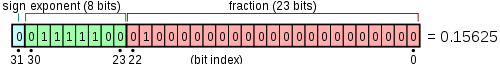
\includegraphics[scale=0.66]{structs/500px-Float_example.png}
\caption{\IFRU{Формат значения float (иллюстрация взята из wikipedia)}
{float value format (illustration taken from wikipedia)}}
\end{figure}

\lstinputlisting{structs/15_2_en.c}

\IFRU{Структура \TT{float\_as\_struct} занимает в памяти столько же места сколько и \Tfloat, 
то есть 4 байта или 32 бита.}
{\TT{float\_as\_struct} structure occupies as much space is memory as \Tfloat, e.g., 4 bytes or 32 bits.}

\IFRU{Далее мы выставляем во входящем значении отрицательный знак, 
а также прибавляя двойку к экспоненте, мы тем 
самым умножаем всё значение на \TT{$2^2$}, то есть на 4.}
{Now we setting negative sign in input value and also by addding 2 to exponent we thereby multiplicating
the whole number by \TT{$2^2$}, e.g., by 4.}

\IFRU{Компилируем в MSVC 2008 без оптимизации:}{Let's compile in MSVC 2008 without optimization:}

\IFRU{\lstinputlisting{structs/15_2_msvc_ru.asm}}{\lstinputlisting{structs/15_2_msvc_en.asm}}

\IFRU{Слекга избыточно. В версии скомпиленной с флагом \Ox нет вызовов \TT{memcpy()}, 
там работа происходит сразу с переменной f. Но по неоптимизированной версии будет проще понять.}
{Redundant for a bit. If it compiled with \Ox flag there are no \TT{memcpy()} call,
f variable is used directly. But it's easier to understand it all considering unoptimized version.}

\IFRU{А что сделает GCC 4.4.1 с опцией \TT{-O3}?}{What GCC 4.4.1 with \TT{-O3} will do?}

\lstinputlisting{\IFRU{structs/15_2_gcc_O3_ru.asm}{structs/15_2_gcc_O3_en.asm}}

\IFRU{Да, функция \TT{f()} в целом понятна. Однако, что интересно, еще при компиляции, 
не взирая на мешанину с полями структуры, GCC умудрился вычислить результат функции \TT{f(1.234)} и 
сразу подставить его в аргумент для \printf{}!}
{The \TT{f()} function is almost understandable. However, what is interesting, GCC was able to calculate
\TT{f(1.234)} result during compilation stage despite all this hodge-podge with structure fields
and prepared this argument to \printf{} as precalculated!}

